\section{Konstrukcja interpolujących sześciennych funkcji sklejanych}
	
	\begin{frame}{Konstrukcja interpolujących sześciennych funkcji sklejanych}

     Ponieważ $s_i(x)$ - sześcienna, \\
     	  to $s''_i(x)$ -liniowa na przedziale $[x_{i},x_{i+1}] $\\
	 wprowadzam $h_{i}=x_{i+1}-x_{i}$, wtedy (z (*)):\\
	 \vspace{3mm}
	   \begin{center}
	  $s_i^{''}(x)=s_i^{''}(x_i)\frac{x_{i+1}-x}{h_i}+s_i^{''}(x_{i+1})\frac{x-x_i}{h_i}$(**)\\
	  	  \end{center}
	  całkując dwukrotnie otrzymuję:\\
	  \begin{center}
	       $s_i(x)=\frac{s_i^{''}(x_i)}{6h_i}(x_{i+1}-x)^3+\frac{s_i^{''}(x_{i+1})}{6h_i}(x-x_i)^3+C(x-x_i)+D(x_{i+1}-x)$, 
	  \end{center}
	   gdzie C, D - stałe całkowania.\\
	  korzystając z  warunków interpolacji :\\
	  $s_i(x_i)=y_i$ oraz $s_i(x_{i+1})=y_{i+1}$ mogę wyliczyć C i D 
	  	\end{frame}
	  \begin{frame}
	   Po wyliczeniu C i D z  warunków interpolacji mamy:\\
	  $s_i(x)=\frac{s_i^{''}(x_i)}{6h_i}(x_{i+1}-x)^3+\frac{s_i^{''}(x_{i+1})}{6h_i}(x-x_i)^3+
	  (\frac{y_{i+1}}{h_i}-\frac{s_i^{''}(x_{i+1})h_i}{6})(x-x_i)+(\frac{y_i}{h_i}-\frac{s_i^{''}(x_{i})h_i}{6})(x_{i+1}-x)$  \\
		 \vspace{3mm}
	 W powyższym wzorze nie znamy $s_i^{''}(x)$ . Aby je wyliczyć korzystamy z warunku ciągłości pierwszej pochodnej. Różniczkujemy więć $s_i(x)$\\
	 	 \vspace{3mm}
	 $s_i^{'}(x_i)=-\frac{h_i}{3}s_i^{''}(x_i)-\frac{h_i}{6}s_i^{''}(x_{i+1})-\frac{y_i}{h_i}+\frac{y_{i+1}}{h_i}$\\
	 	 \vspace{3mm}
	    Dla przejrzystości wprowadzamy symbole: $\sigma_{i}=\frac{1}{6}s''(x_{i})$ oraz $\Delta_{i}=\frac{y_{i+1}-y_{i}}{h_{i}} $ (uwaga: $\Delta$ oznacza co innego niż na poprzednim wykładzie), wtedy: \\
	     \vspace{3mm}
	    $s_i^{'}(x_i)=-2\sigma_{i}h_i-\sigma_{i+1}h_i+\Delta_{i}$\\
        $ s_{i}'(x_{i})  &=\ \Delta_{i}-h_{i}(\sigma_{i+1}+2\sigma_{i})$\\
        Natomiast    od drugiej strony:\\   	
        $s_{i-1}'(x_{i}) &=\ \Delta_{i-1}+h_{i-1}(2\sigma_{i}+\sigma_{i-1})$\\
        \end{frame}
        
        
        
        \begin{frame}
        \begin{block}{}
        	\centering Warunek ciągłości: $s_{i-1}'(x_{i}) = s_{i}'(x_{i})$
        \end{block}
        \[
        	\framebox{$\Delta_{i-1}+h_{i-1}(2\sigma_{i}+\sigma_{i-1})=
            \Delta_{i}-h_{i}(\sigma_{i+1}+2\sigma_{i})$}
        \]
        otrzymujemy układ (n-2) równań liniowych  (dla punktów pośrednich):
        \[
        	h_{i-1}\sigma_{i-1}+2(h_{i-1}+h_{i})\sigma_{i}+h_{i}\sigma_{i+1}=
            \Delta_{i}-\Delta_{i-1}, \ \ i=2, 3, . . . , n-1
        \]
        ale ponieważ mamy n niewiadomych $\sigma_{i}$ konieczne jest
        określanie dwóch dodatkowych warunków.
    \end{frame}
    %%%%%%%%%%%%%%%%%%%%%%%
    \begin{frame}
		$\newline$
    	Istnieje wiele sposobów określania dodatkowych warunków.
       \begin{enumerate}
       \item  \[
		\begin{rcases*}
			C_{1}(x) - \textrm{f. sześcienna przez pierwsze 4 punkty}\\
			C_{n}(x) - \textrm{f. sześcienna przez ostatnie 4 punkty}
		\end{rcases*} \rightarrow
		\]	
       \end{enumerate}	
       \[
       		\framebox{$s'''(x_{1})=C^{'''}_{1}\ \ \ s'''(x_{n})=C^{'''}_{n}$}
       \]
        Stałe $C^{'''}_{1}$ i $C^{'''}_{n}$ mogą być określone bez znajomości 
        $C_{1}(x)$ i $C_{n}(x)$:
        \[
        	\Delta_{i}\ =\ \frac{y_{i+1}-y_{i}}
            {x_{i+1}-x_{i}}\ ;\ \textrm{przybliża 1-szą pochodną}
        \]
        \[
        	\Delta_{i}^{(2)}=\frac{\Delta_{i+1}-\Delta_{i}}
            {x_{i+2}-x_{i}}\ ;\ 2\Delta_{i}^{(2)}\approx f^{''}
        \]
        \[
        	\Delta_{i}^{(3)}\ =\ \frac{\Delta_{i+1}^{(2)}-\Delta_{i}^{(2)}}
            {x_{i+3}-x_{i}}\ ;\ 6\Delta_{i}^{(3)}\approx f^{'''}
        \]
    \end{frame}
    %%%%%%%%%%%%%%%%%%%%%%
    \begin{frame}
    	i ogólnie dla ilorazów róznicowych:
        \begin{flushright}
        	$\Delta_{0}^{(0)}=f[x_{0}]\equiv f(x_{0}) \linebreak \linebreak$
            $\Delta_{0}^{(1)}=f[x_{0},\ x_{1}]\equiv\frac{f[x_{1}]-f[x_{0}]}{x_{1}-
            x_{0}}=\frac{f(x_{1})-f(x_{0})}{x_{1}-x_{0}} 
            \linebreak \linebreak$
            $\Delta_{0}^{(3)}=f[x_{0},\ x_{1},\ x_{2}]\equiv\frac{f[x_{1},x_{2}]-f[x_{0},x_{1}]}
            {x_{2}-x_{0}} \linebreak $
            $\ldots \ldots \linebreak$
            $\Delta_{0}^{(n)}=f[x_{0},\ x_{1},\ .\ .\ .\ ,\ x_{k}]\equiv\frac{f[x_{1},\ldots,x_{k}]-f[x_{0},\ldots,x_{k-1}]}{x_{k}-x_{0}}$
        \end{flushright}
        mamy związek między ilorazami różnicowymi a pochodnymi:
        \begin{exampleblock}{}
        	$
            	\centering f[x_{0}, ... \ , x_{n}]=\frac{f^{(n)}(\eta)}
                {n!}, \ \ \ \eta \in [x_{0},... \ , x_{n}]
                \ \ \ (\eta \textrm{- pewien punkt})
            $
        \end{exampleblock}
        \begin{block}{Przypomnienie}
         To wynika z 	uogólnionego  twierdzenie o wartości średniej (poprzedni wykład) 
        \end{block}
        
    \end{frame}
    %%%%%%%%%%%%%%
    \begin{frame}
    	Różniczkując wzór na $s^{''}(x)$ w przedziale $[x_{i},x_{i+1}] $ (**) otrzymujemy:
        $s_i^{'''}(x)=\frac{-s_i^{''}(x_i)}{h_i}+\frac{s_i^{''}(x_{i+1})}{h_i}=\frac{-6\sigma_{i}}{h_i}+\frac{6\sigma_{i+1}}{h_i}$\\
        Wtedy:
        \begin{align*}
        	s'''(x_{1})&=c_{1}'''(x_{1}) \Rightarrow
            \frac{6}{h_{1}}(\sigma_{2}-\sigma_{1})=6\Delta_{1}^{(3)}
            &|\cdot h_{1}^{2}
            \\
            s'''(x_{n})&=c_{n}'''(x_{1}) \Rightarrow
            \frac{6}{h_{n-1}}(\sigma_{n}-\sigma_{n-1})=6\Delta_{n-3}^{(3)}
            &|\cdot h_{n-1}^{2}
        \end{align*}
        po przekształceniu: (cel = symetria)
        $\newline \newline
        \begin{cases}
        	-h_{1}\sigma_{1}+h_{1}\sigma_{2}=h_{1}^{2}\Delta_{1}^{(3)}
            \\
		h_{n-1}\sigma_{n-1}-h_{n-1}\sigma_{n}=-h_{n-1}^{2}\Delta_{n-3}^{(3)}
        \end{cases}
        $
    \end{frame}
    %%%%%%%%%%%%%%%%%%
    \begin{frame}
    	mamy:
        \[
        \begin{bmatrix}
    -h_{1} & h_{1} & 0 & 0  & 0 \\
    h_{1} & 2(h_{1}+h_{2}) & h_{2} & 0  & 0 \\
    0 & h_{2} & 2(h_{2}+h_{3}) & h_{3} & 0 \\
    \vdots & \vdots & \vdots & \vdots & \vdots \\
    0 & 0 & h_{n-2} & 2(h_{n-2}+h_{n-1}) & h_{n-1} \\
    0 & 0 & 0 & h_{n-1}  & -h_{n-1}
		\end{bmatrix}
        \begin{bmatrix}
        	\sigma_{1} \\
            \sigma_{2} \\
            \sigma_{3} \\
            \vdots \\
            \sigma_{n-1} \\
            \sigma_{n}
        \end{bmatrix}
       	=
        \]
        \[	=
        	\begin{bmatrix}
        		h_{1}^{2}\Delta^{(3)}_{1} \\
                \Delta_{2} - \Delta_{1} \\
                \Delta_{3} - \Delta_{2} \\
                \vdots \\ 
                \Delta_{n-1} - \Delta_{n-2} \\
                -h_{n-1}^{2}\Delta^{(3)}_{n-3}
        	\end{bmatrix}
        \]
    \end{frame}
    %%%%%%%%%%%%%%%%%%
    \begin{frame}{Inne ważne możliwości określania warunków}
    	\begin{itemize}
    		\item natural cubic spline: $s''(x_{1})=s''(x_{n})=0$ (free boundary)
            \item clamped boundary: $s'(x_{1})=f'_{1}, \ \ s'(x_{n})=f'_{n}$ (pierwsze pochodne na krańcach znane bądź przybliżone ilorazami różnicowymi)
            \item $s''(x_{1})=y''_{1}; \ \ s^{n}(x_{n})=y''_{n}$ (drugie pochodne na krańcach znane bądź przybliżone ilorazami różnicowymi, szczególny przypadek to natural cubic splines)
            \item not-a-knot condition $s'''_1(x_2)=s'''_2(x_2)$ oraz $s'''_{n-1}(x_{n-1})=s'''_{n}(x_{n-1})$  czyli $s'''(x)$ ciągła w $x_{2}$ oraz $x_{n-1}$
            \item interpolowanie spline'ami funkcji periodycznych
            $s(x_1)=s(x_n)$,
            $s'(x_1)=s'(x_n)$ oraz
            $s^{''}(x_1)=s^{''}(x_n)$
    	\end{itemize}
    \end{frame}
    %%%%%%%%%%%%%%%%%%%%
    \begin{frame}{Clamped boundary condition}
   
        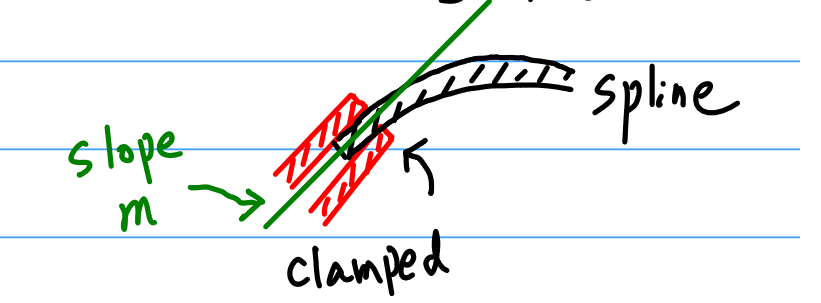
\includegraphics[width=0.7\textwidth]{img/4/clamped.png}
        
         źródło: \url{http://runge.math.smu.edu/HiPerfSciComp/_downloads/CubicSpline.pdf}
    \end{frame}
    \begin{frame}
    
        	Dla obliczeń - zwłaszcza wielokrotnego określania wartości s(x) 
            korzystna jest postać:
            \[
            	s(x)=y_{i}+b_{i}\cdot(x-x_{i})+c_{i}
                \cdot(x-x_{i})^{2}+d_{i}\cdot(x-x_{i})^{3}
                \ \ dla \ x\in[x_{i},\ x_{i+1}]
            \]
            $b_{i}, c_{i}, d_{i}$ - określone dla każdego przedziału:
            $b_{i}=\frac{y_{i+1}-y_{i}}{h_{i}}-h_{i}\cdot (\sigma_{i+1}
            +2\sigma_{i})\newline$
            $c_{i}=3\cdot \sigma_{i}\newline$
            $d_{i}=\frac{\sigma_{i+1}-\sigma_{i}}{h_{i}}\newline$

        
    \end{frame}
    %%%%%%%%%%%%%%%%%%%%
    \begin{frame}{Błąd interpolacji funkcji sklejanych}
    	Przykładowo dla {\it clamped boundary condition} udowodniono :
        \begin{itemize}
        \item $a=x_{1}, x_{2}, . . . , x_{n}=b$
        \item $f\in C^{4}[a,\ b] , \ \ \ \ \max_{x\in[a,b]}|f^{(4)}
        (x)|\leq M$
        \item $s'(x_{1})=f'(x_{1}), \ \ \ s'(x_{n})=f'(x_{n})$
        \end{itemize}
        to:
        \[
        	\max_{x\in[a,b]}|f(x)-s(x)|\leq \frac{5}{384} \cdot
            M \cdot \max_{1 \leq i \leq n-1}(x_{i+1}-x_{i})^{4}
        \]
        
        Wniosek:  jeśli dodamy 10 razy więcej punktów intepolacji, długość przedziału 
        $x_{i+1}-x_{i}$ zmniejszy się 10-krotnie, a ograniczenie górne błedu zmniejszy się $10^4$ razy !\\
        \small{
        Dowód A. Hall, W. Weston Meyer "Optimal error bounds for cubic spline interpolation",  \url{https://www.sciencedirect.com/science/article/pii/002190457690040X})}
    \end{frame}
    
    
    
    
    
    
    
    
    
    
    
    
    
    
    
    
    
    
    
    
    
    

    
    
    
    
    
    
    
    
    
    
    
    
    
    
    
    
    
    
    